\fancyhead{}
\fancyfoot{}
\cfoot{\thepage}

\lhead{Resultados}

\chapter{Resultados}

Para garantizar resultados precisos durante la evaluación del sistema de asistencia basado en reconocimiento facial, se definió un entorno de pruebas controlado. A continuación, se detallan las características del hardware y software utilizados, así como la versión del sistema y los módulos activados durante las pruebas.

\section{Figuras y Tablas}

\begin{table}[H]
    \centering
    \caption{Componentes de hardware y software utilizados en el sistema}
    \label{tab:entorno_pruebas}
    \renewcommand{\arraystretch}{1.3}
    \begin{tabular}{|p{5cm}|p{9cm}|}
        \hline
        \textbf{Elemento} & \textbf{Descripción} \\
        \hline
        Modelo de cámara & cámara web HD 720p \\
        \hline
        Servidor & AMD Ryzen 7 7735HS, 16 GB RAM, SSD 512 GB, Windows 11 Home 	\\
        \hline
        Librerías & OpenCV,numpy, ultralytics,deepface,tensorflow-cpu==2.13.0,omegaconf\\
        \hline
        Lenguaje de programación & Python 3.8.10 \\
        \hline
        Versión del sistema desarrollado & v1.0 Beta \\
        \hline
        Módulos activados & Captura de imagen, Preprocesamiento, Detección, Reconocimiento, Registro en base de datos \\
        \hline
    \end{tabular}
\end{table}


\subsection{Errores detectados y ajustes aplicados}

Durante la etapa de pruebas, se identificaron ciertos errores recurrentes en el funcionamiento del sistema, principalmente relacionados con la precisión del reconocimiento facial. A continuación, se presenta una tabla con los tipos de errores detectados, su causa y las acciones de mitigación implementadas para mejorar el desempeño.

\begin{table}[H]
    \centering
    \caption{Errores frecuentes y acciones de mitigación}
    \label{tab:errores_ajustes}
    \renewcommand{\arraystretch}{1.3}
    \begin{tabular}{|p{4cm}|p{6cm}|p{4.5cm}|}
        \hline
        \textbf{Tipo de error} & \textbf{Causa identificada} & \textbf{Ajuste o solución aplicada} \\
        \hline
        Falsos positivos en la identificación facial & Umbral de similitud fijo (50) no adecuado para la variabilidad de datos por usuario & Se ajustó el umbral dinámicamente según la cantidad de imágenes por usuario y su variación interna \\
        \hline
        Reconocimiento erróneo con poca iluminación & Capturas de imágenes en condiciones de baja luz o sombras parciales & Se incorporó preprocesamiento de imagen (mejora de contraste y normalización) \\
		\hline
		Procesamiento lento con gran volumen de usuarios & Comparación secuencial con todos los embeddings registrados & Se implementó filtrado previo por clase probable y limitación del número de comparaciones activas \\
		\hline
    \end{tabular}
\end{table}

\begin{table}[H]
\centering
\caption{Configuración de umbral vs. resultado esperado}
\label{tab:umbral_similitud}
\renewcommand{\arraystretch}{1.3}
\scriptsize
\begin{tabular}{|c|c|p{3.5cm}|p{5cm}|}
\hline
\textbf{Umbral ($\texttt{min\_dist} >$ ?)} & \textbf{Factor de similitud} & \textbf{Resultado esperado} & \textbf{Notas} \\
\hline
$> 1.0$ & $100 - \texttt{dist} \times 30$ & Reconocimiento muy estricto & Muy preciso, pero puede fallar si la luz o ángulo cambia \\
\hline
$> 1.3$ & $100 - \texttt{dist} \times 25$ & Recomendado en entornos controlados & Balance entre precisión y tolerancia \\
\hline
$> 1.8$ & $100 - \texttt{dist} \times 20$ & Reconoce con más flexibilidad & Acepta diferencias de expresión o iluminación \\
\hline
$> 3.5$ & $100 - \texttt{dist} \times 18$ & Tolerante, puede haber falsos positivos & Útil si los embeddings fueron generados con solo 1 o 2 imágenes \\
\hline
$> 5.0$ & $100 - \texttt{dist} \times 15$ & Muy laxo, reconoce casi todo & Solo útil para pruebas \\
\hline
$> 10.0$ & $100 - \texttt{dist} \times 10$ & \textbf{Demasiado permisivo} & Como en su captura: reconoce a cualquiera con similitud muy baja \\
\hline
\end{tabular}
\end{table}


\subsection{Configuraciones aplicadas y resultados obtenidos}

\textbf{Configuración 1: Umbral 1.0 y factor 30}

\begin{figure}[H]
    \centering
    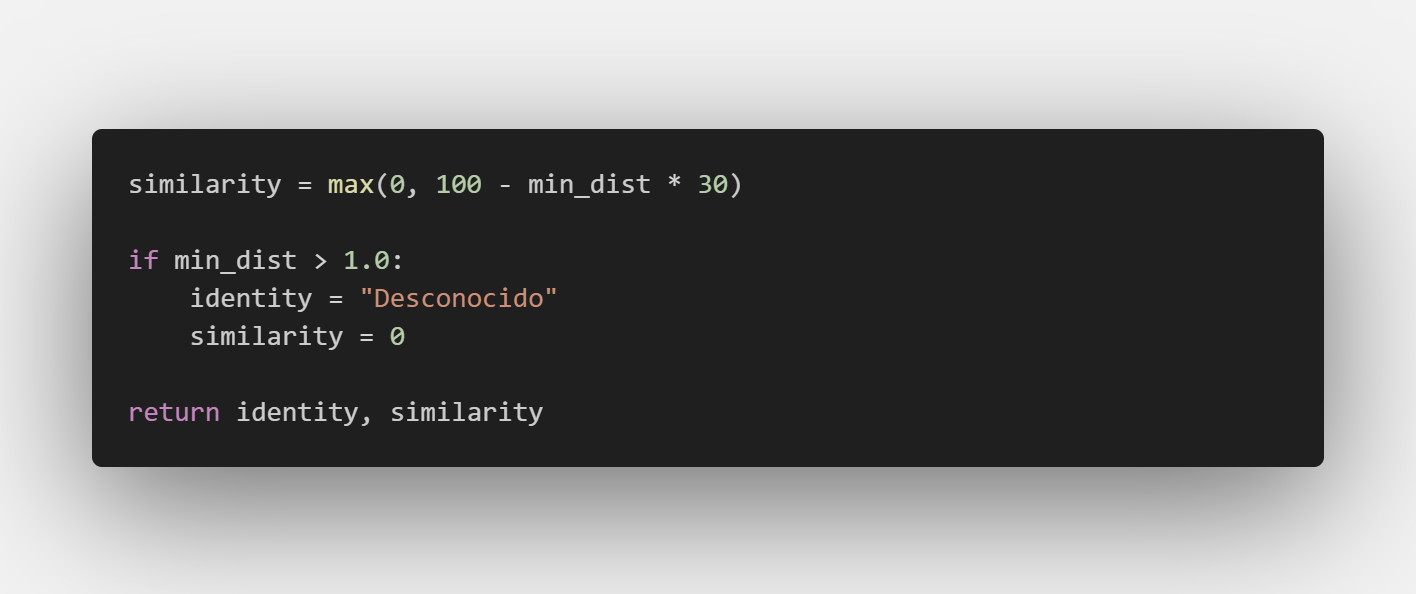
\includegraphics[width=0.8\textwidth]{capitulo_04/imagenes/1.jpg}
    \caption{Fragmento de código utilizado para configurar el umbral de reconocimiento facial.}
\end{figure}

\begin{figure}[H]
    \centering
    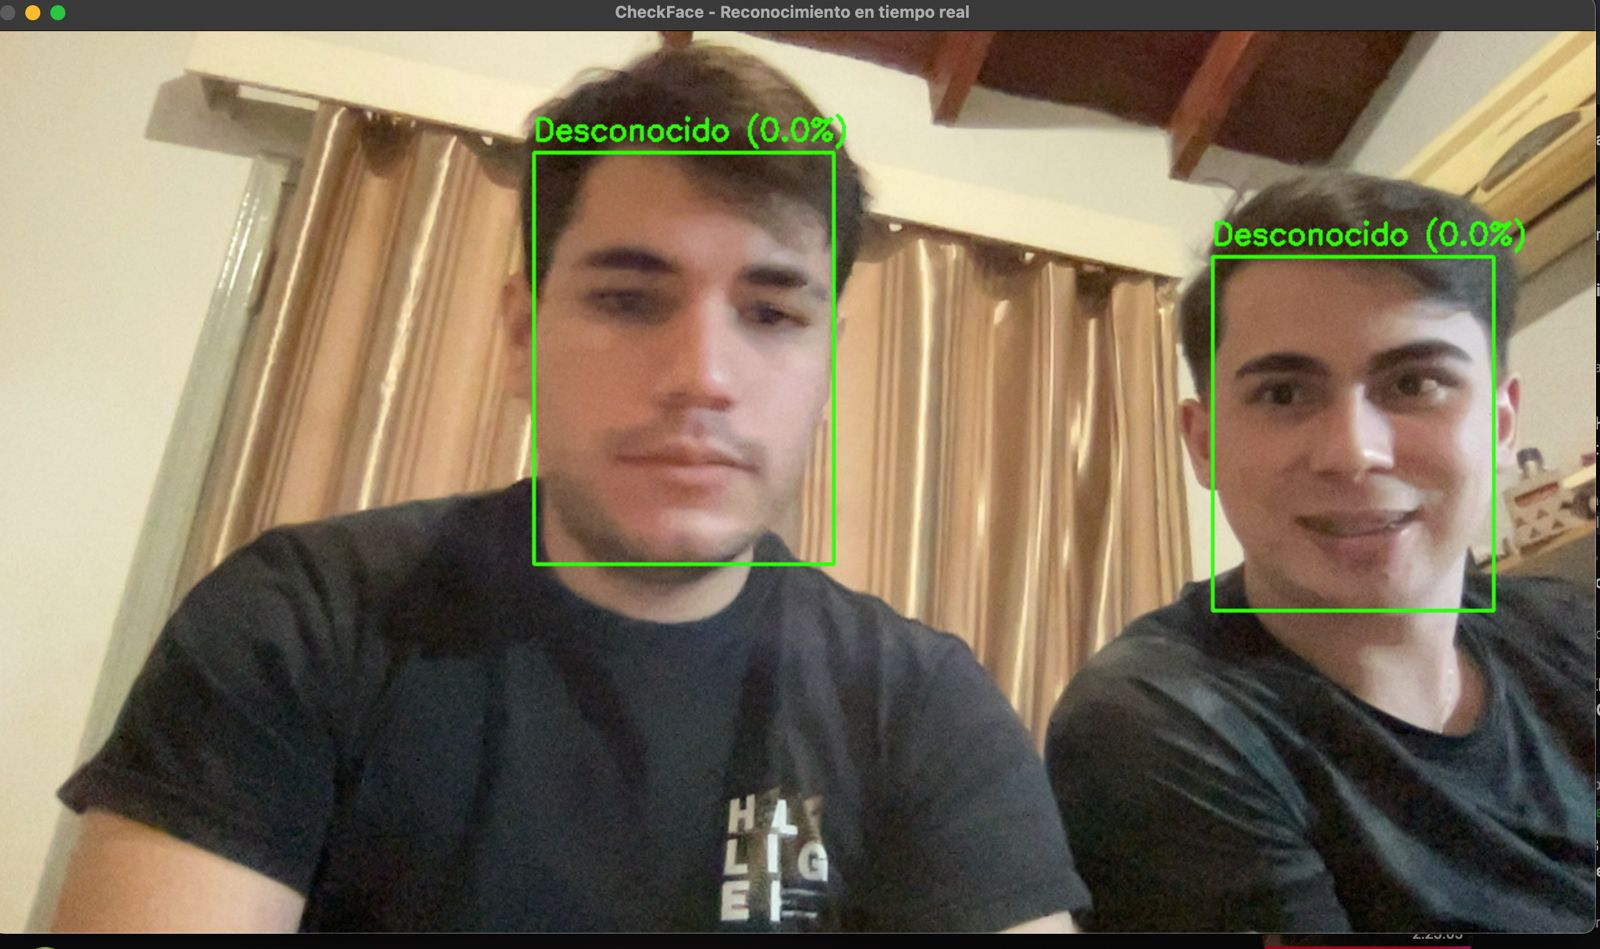
\includegraphics[width=0.8\textwidth]{capitulo_04/imagenes/umbral_1.0_30.jpg}
    \caption{Resultados obtenidos aplicando la configuración anterior (umbral = 1.0 y factor de similitud 30).}
\end{figure}

\newpage

\textbf{Configuración 2: Umbral 1.3 y factor 25}

\begin{figure}[H]
    \centering
    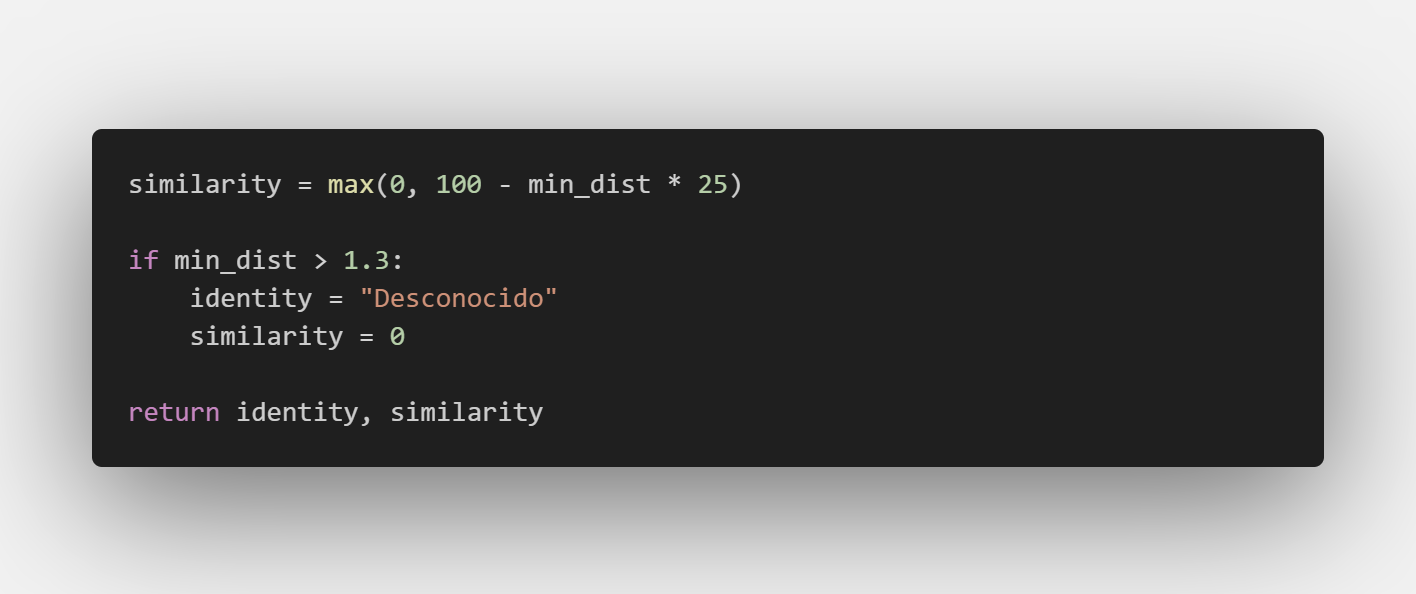
\includegraphics[width=0.8\textwidth]{capitulo_04/imagenes/2.png}
    \caption{Fragmento de código utilizado para configurar el umbral de reconocimiento facial.}
\end{figure}

\begin{figure}[H]
    \centering
    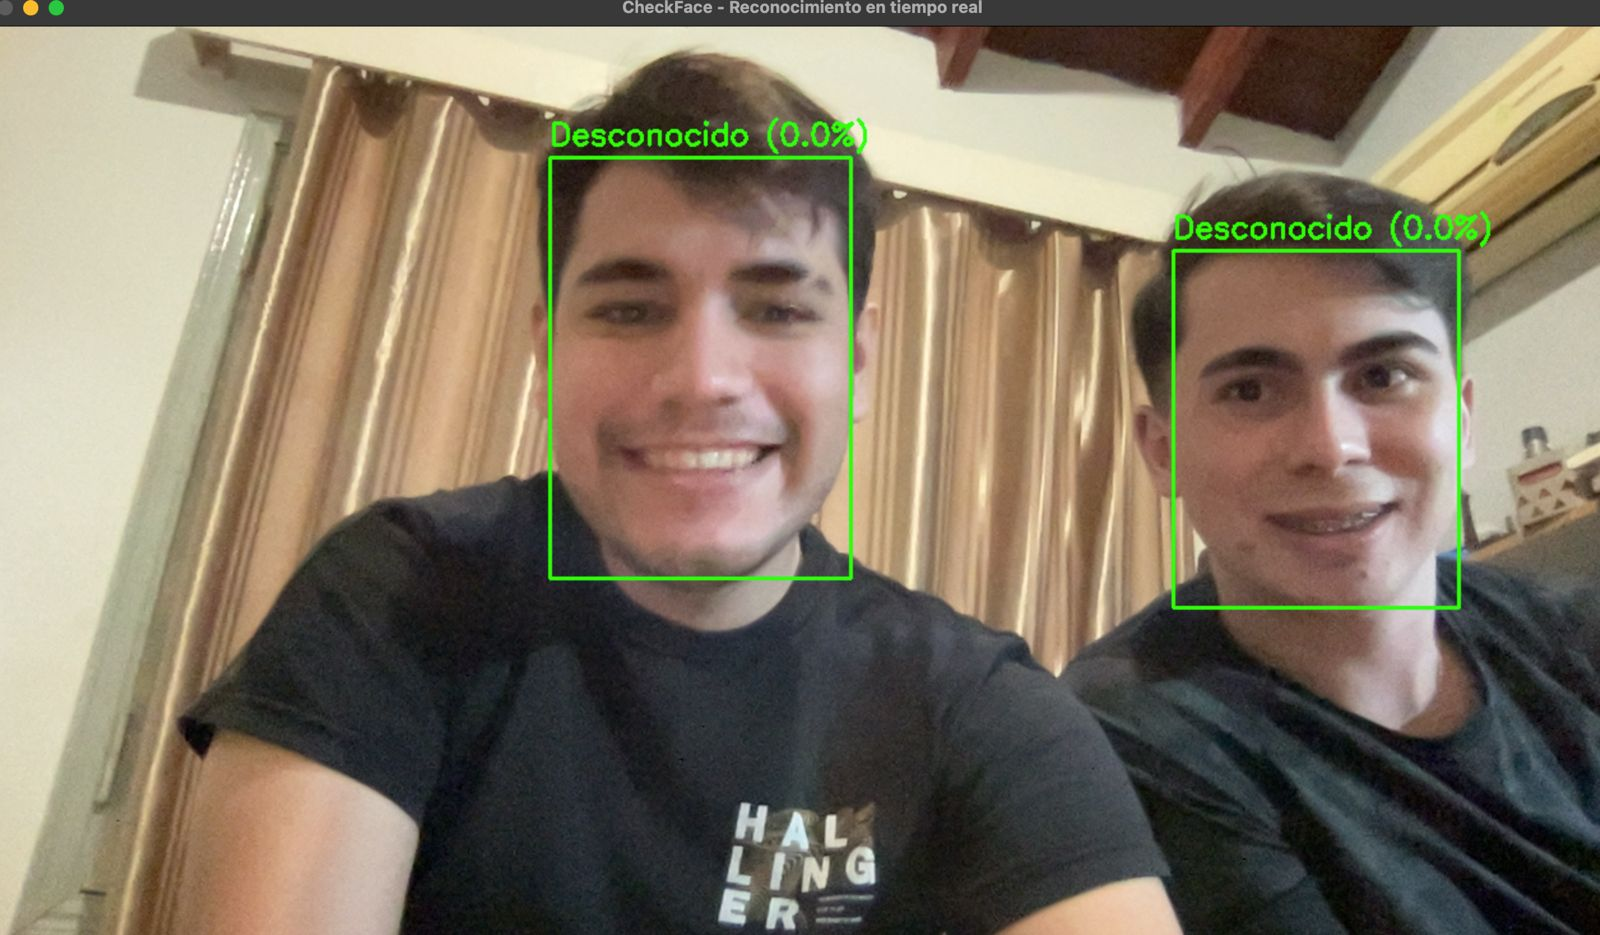
\includegraphics[width=0.8\textwidth]{capitulo_04/imagenes/1.3_min_dist25.jpg}
    \caption{Resultados obtenidos aplicando la configuración anterior (umbral = 1.3 y factor de similitud 25).}
\end{figure}

\newpage

\textbf{Configuración 3: Umbral 1.8 y factor 20}

\begin{figure}[H]
    \centering
    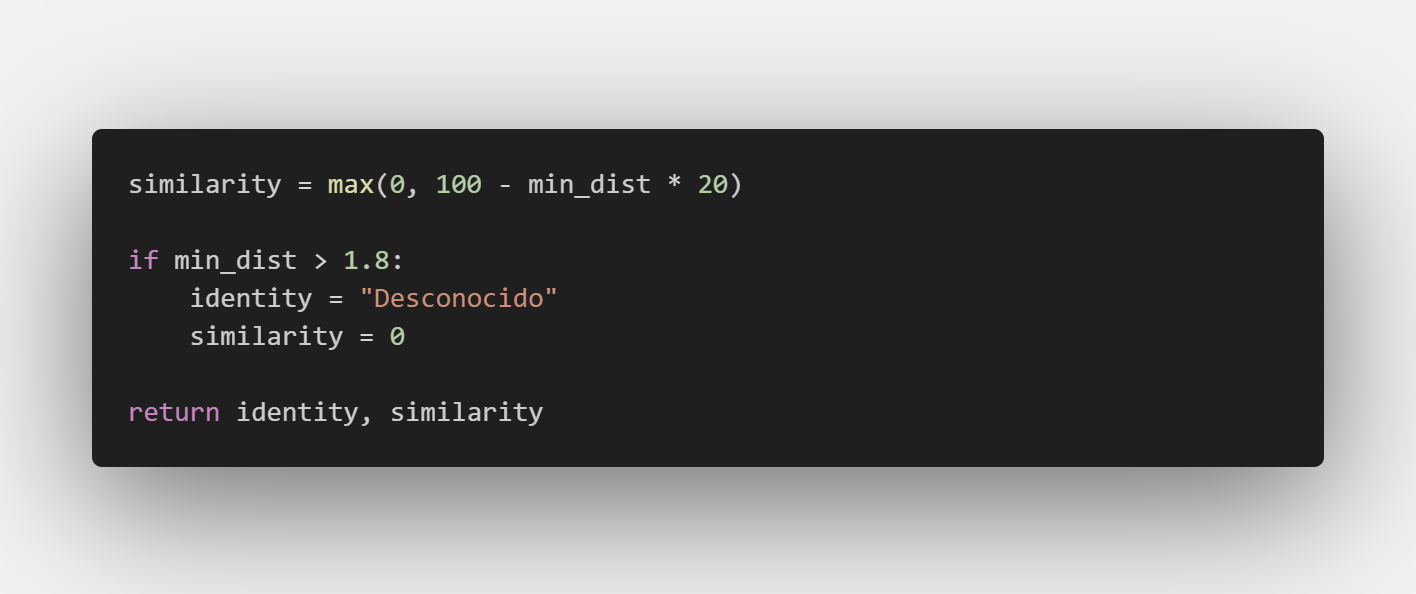
\includegraphics[width=0.8\textwidth]{capitulo_04/imagenes/3.png}
    \caption{Fragmento de código utilizado para configurar el umbral de reconocimiento facial.}
\end{figure}

\begin{figure}[H]
    \centering
    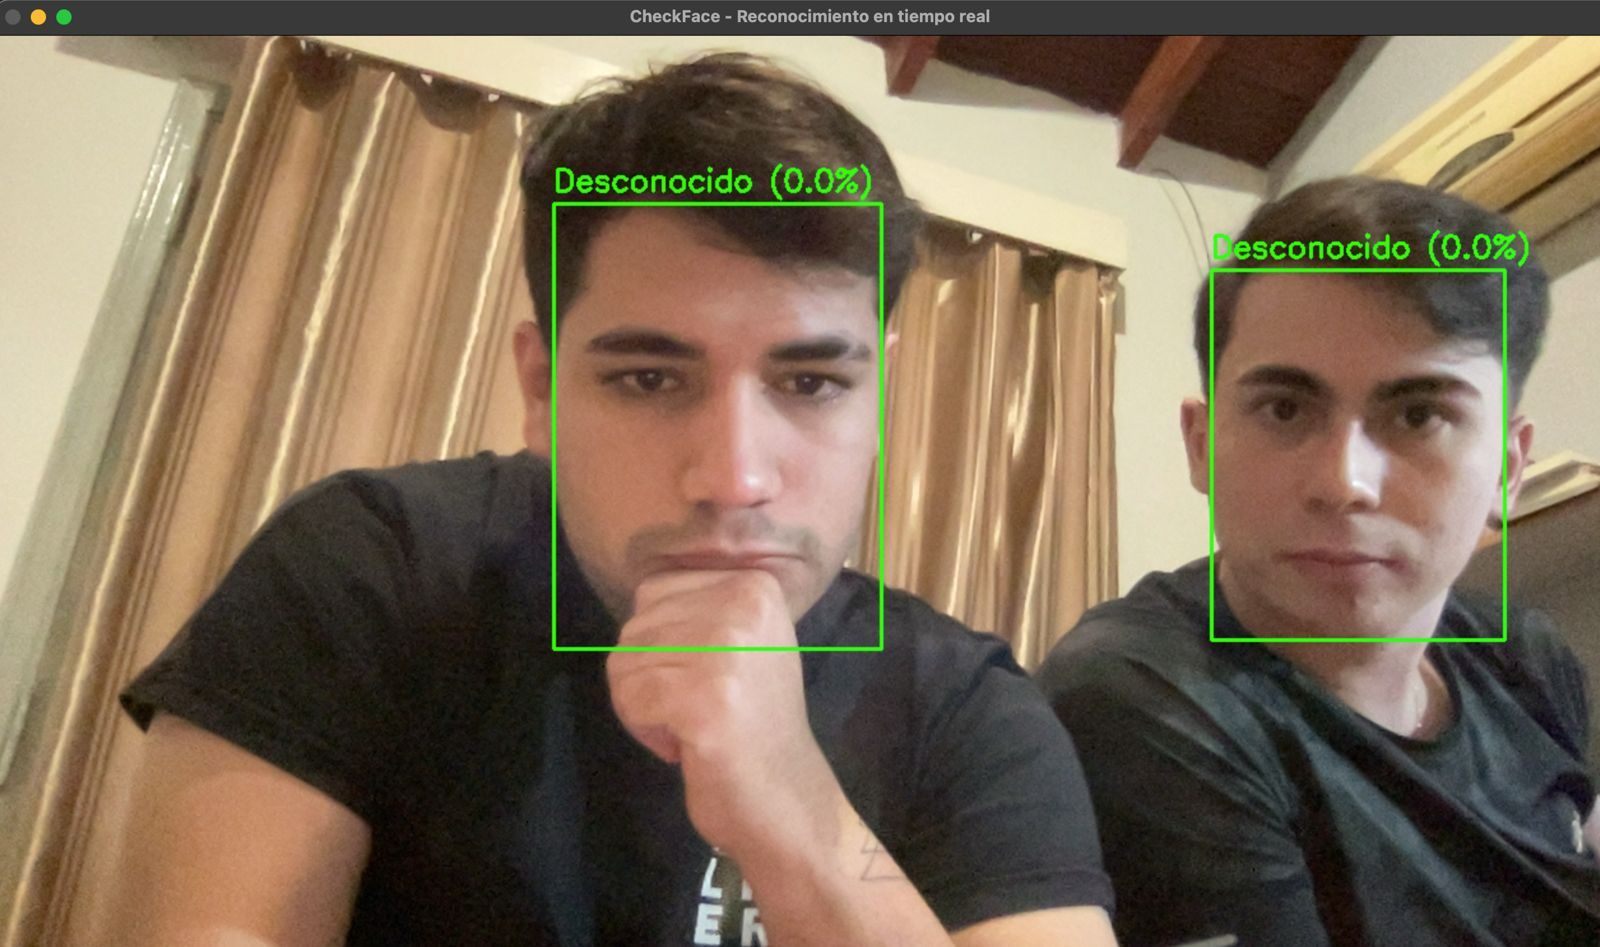
\includegraphics[width=0.8\textwidth]{capitulo_04/imagenes/umbral1.8min_dist20.jpg}
    \caption{Resultados obtenidos aplicando la configuración anterior (umbral = 1.8 y factor de similitud 20).}
\end{figure}

\newpage


\textbf{Configuración 4: Umbral 3.5 y factor 18}

\begin{figure}[H]
    \centering
    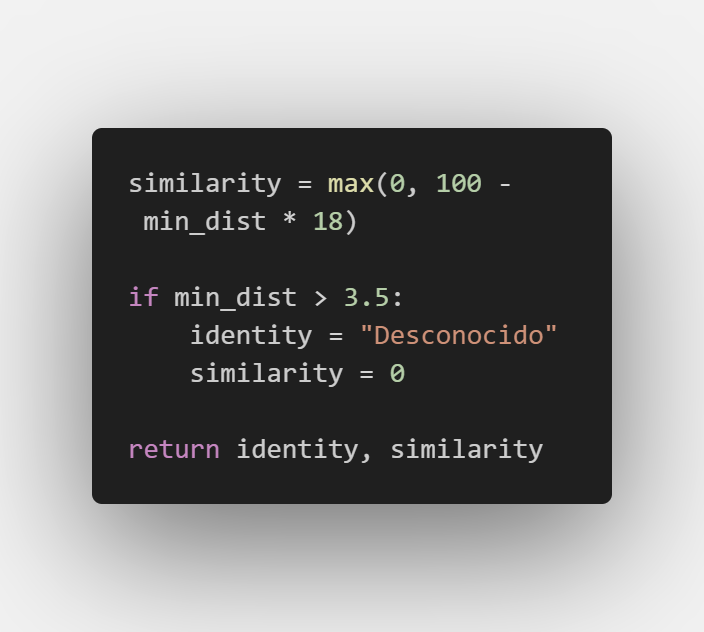
\includegraphics[width=0.8\textwidth]{capitulo_04/imagenes/4.png}
    \caption{Fragmento de código utilizado para configurar el umbral de reconocimiento facial.}
\end{figure}

\begin{figure}[H]
    \centering
    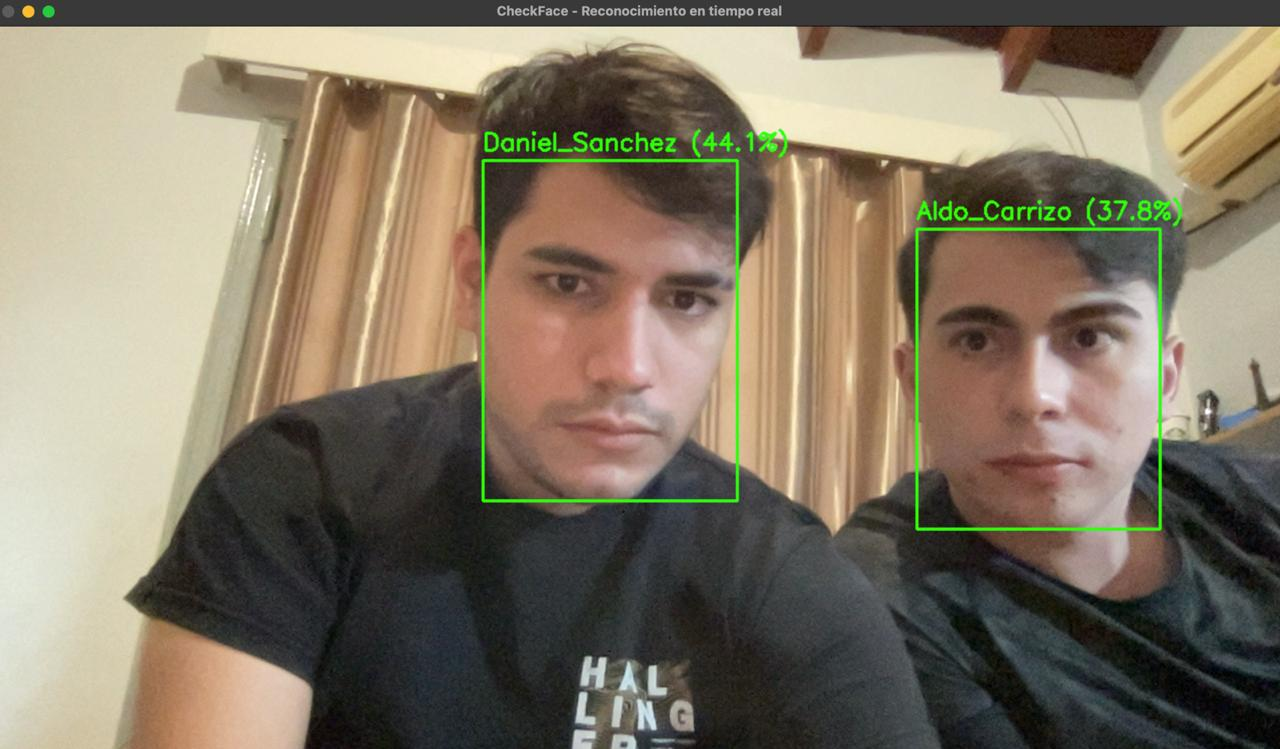
\includegraphics[width=0.8\textwidth]{capitulo_04/imagenes/4.4.jpg}
    \caption{Resultados obtenidos aplicando la configuración anterior (umbral = 3.5 y factor de similitud 18).}
\end{figure}


\newpage


\textbf{Configuración 5: Umbral 5 y factor 15}

\begin{figure}[H]
    \centering
    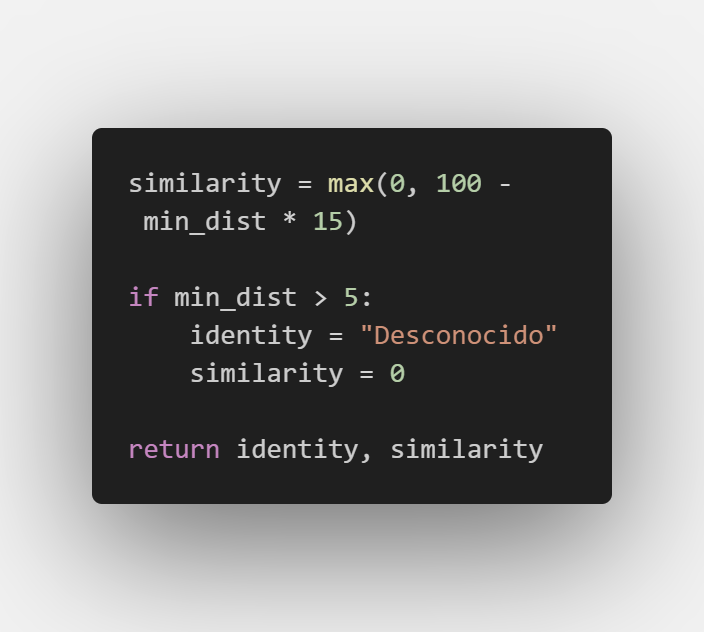
\includegraphics[width=0.8\textwidth]{capitulo_04/imagenes/5.png}
    \caption{Fragmento de código utilizado para configurar el umbral de reconocimiento facial.}
\end{figure}

\begin{figure}[H]
    \centering
    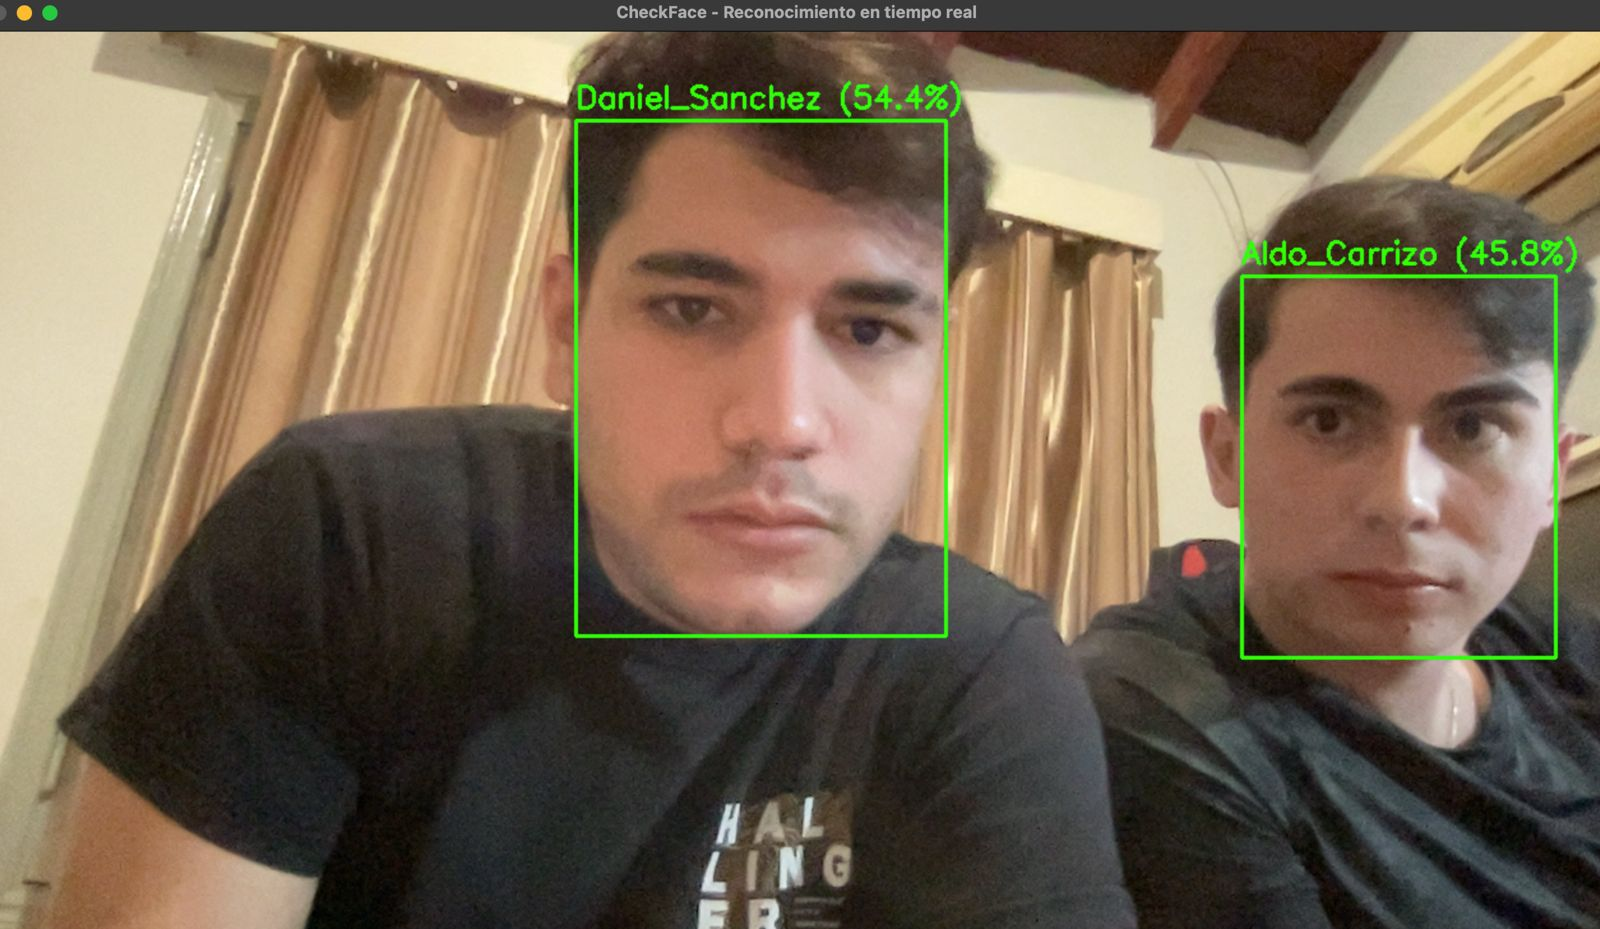
\includegraphics[width=0.8\textwidth]{capitulo_04/imagenes/5.5.jpg}
    \caption{Resultados obtenidos aplicando la configuración anterior (umbral = 5 y factor de similitud 15).}
\end{figure}


\newpage


\textbf{Configuración 6: Umbral 10 y factor 10}

\begin{figure}[H]
    \centering
    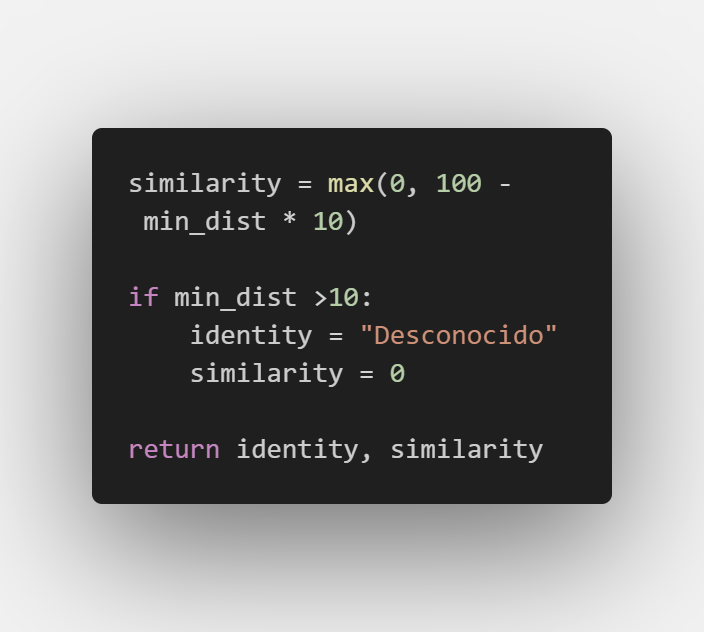
\includegraphics[width=0.8\textwidth]{capitulo_04/imagenes/6.png}
    \caption{Fragmento de código utilizado para configurar el umbral de reconocimiento facial.}
\end{figure}

\begin{figure}[H]
    \centering
    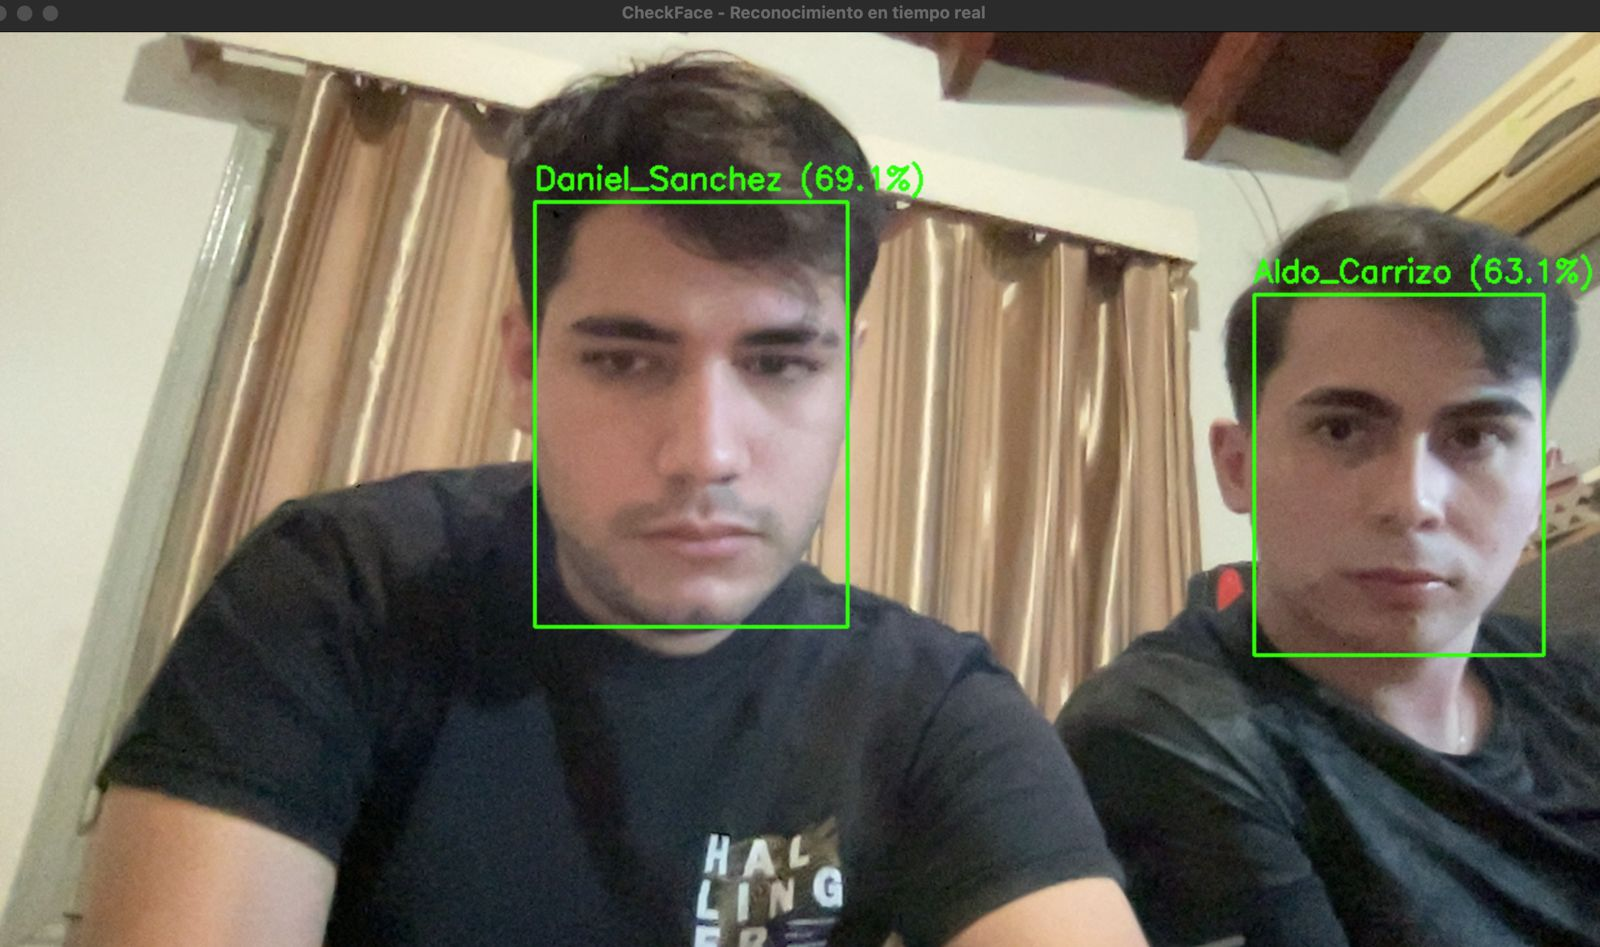
\includegraphics[width=0.8\textwidth]{capitulo_04/imagenes/6.6.jpg}
    \caption{Resultados obtenidos aplicando la configuración anterior (umbral = 10 y factor de similitud 10).}
\end{figure}






\subsubsection*{Comparativa de modelos YOLO para detección facial}

Se evaluaron diferentes versiones de YOLO adaptadas al reconocimiento facial. Finalmente, se seleccionó YOLOv8n-Face por su buen equilibrio entre precisión, velocidad y soporte de keypoints.


\begin{table}[H]
    \centering
    \caption{Comparativa de modelos YOLO para detección facial}
    \label{tab:comparativa_yolo}
    \renewcommand{\arraystretch}{1.3}
    \scriptsize
    \begin{tabular}{|p{3cm}|p{2.3cm}|p{1.3cm}|p{1.3cm}|p{1.3cm}|p{4.5cm}|}
        \hline
        \textbf{Modelo} & \textbf{mAP@0.5:0.95} & \textbf{Precisión} & \textbf{Recall} & \textbf{Velocidad (ms/img)} & \textbf{Observaciones} \\
        \hline
        YOLOv5n-Face & $\sim$0.31 & $\sim$0.60 & $\sim$0.35 & $\sim$2.1 & Ligero y rápido, pero menos preciso. No soporta keypoints. \\
        \hline
        YOLOv5s-Face & $\sim$0.34 & $\sim$0.65 & $\sim$0.37 & $\sim$5.7 & Mejor precisión que v5n, pero aún sin soporte de keypoints. \\
        \hline
        YOLOv8n-Face & \textbf{0.375} & \textbf{0.625} & \textbf{0.43} & $\sim$1.0 & Buen balance entre precisión, velocidad y soporte moderno. Soporta keypoints. \\
        \hline
        YOLOv8s-Face & $\sim$0.43 & $\sim$0.70 & $\sim$0.48 & $\sim$1.2 & Alta precisión, ideal si se dispone de más recursos. Soporta keypoints. \\
        \hline
        YOLOv8m-Face & $\sim$0.46 & $\sim$0.72 & $\sim$0.50 & $\sim$1.8 & Muy preciso, aunque más pesado. Soporta keypoints. \\
        \hline
    \end{tabular}
\end{table}



\subsubsection*{Evaluación según dificultad (WIDER Face)}

La tabla muestra el rendimiento de diferentes modelos YOLO-Face bajo tres niveles de dificultad: fácil, medio y difícil. Estas pruebas se basan en el conjunto de datos WIDER Face, donde las condiciones difíciles incluyen rostros pequeños, parcialmente visibles o con iluminación deficiente. Se observa que YOLOv8-Face presenta mayor robustez en entornos desafiantes.

\begin{table}[H]
    \centering
    \caption{Rendimiento de modelos YOLO en distintos niveles de dificultad (WIDER Face)}
    \label{tab:rendimiento_dificultad}
    \renewcommand{\arraystretch}{1.3}
    \scriptsize
    \begin{tabular}{|p{3.5cm}|c|c|c|}
        \hline
        \textbf{Modelo} & \textbf{Easy (\%)} & \textbf{Medium (\%)} & \textbf{Hard (\%)} \\
        \hline
        YOLOv5s–Face & 91.20 & 89.10 & 71.30 \\
        \hline
        YOLOv8n–Face & 93.79 & 91.82 & 79.38 \\
        \hline
        YOLOv8s–Face & 95.13 & 93.62 & 82.90 \\
        \hline
        YOLOv8x–Face & 96.33 & 95.16 & 85.80 \\
        \hline
    \end{tabular}
\end{table}


\subsubsection*{Comparativa de modelos DeepFace}

La tabla muestra distintos modelos compatibles con DeepFace evaluados en cuanto a precisión, velocidad, tamaño, métrica de comparación y sus ventajas y desventajas. Se destaca ArcFace como el más preciso, aunque requiere buen preprocesamiento.




\begin{table}[H]
    \centering
    \caption{Comparativa de modelos de DeepFace (Parte 1)}
    \label{tab:deepface1}
    \renewcommand{\arraystretch}{1.3}
    \scriptsize
    \begin{tabular}{|p{2.3cm}|c|c|c|c|}
        \hline
        \textbf{Modelo} & \textbf{Precisión (LFW)} & \textbf{Velocidad} & \textbf{Tamaño} & \textbf{Métrica} \\
        \hline
        ArcFace & \textbf{99.83\%} & Media & $\sim$68 MB & Cosine / Euclídea \\
        \hline
        VGG-Face & 98.78\% & Lenta & $\sim$500 MB & Cosine \\
        \hline
        Facenet & 99.20\% & Rápida & $\sim$90 MB & Euclídea \\
        \hline
        Facenet512 & 99.25\% & Media & $\sim$125 MB & Euclídea \\
        \hline
        Dlib & 96.00\% & Muy rápida & $\sim$5 MB & Euclídea \\
        \hline
        SFace & 99.65\% & Media & $\sim$100 MB & Cosine \\
        \hline
    \end{tabular}
\end{table}

\vspace{0.5cm}

\begin{table}[H]
    \centering
    \caption{Comparativa de modelos de DeepFace (Parte 2: ventajas y desventajas)}
    \label{tab:deepface2}
    \renewcommand{\arraystretch}{1.3}
    \scriptsize
    \begin{tabular}{|p{2.3cm}|p{5cm}|p{5cm}|}
        \hline
        \textbf{Modelo} & \textbf{Ventajas principales} & \textbf{Desventajas} \\
        \hline
        ArcFace & Muy alta precisión, robusto ante variaciones de edad, pose y luz & Requiere buen preprocesamiento \\
        \hline
        VGG-Face & Modelo original de DeepFace, bien entrenado & Pesado y lento \\
        \hline
        Facenet & Ligero, buena precisión & Menos preciso que ArcFace \\
        \hline
        Facenet512 & Mejor versión de Facenet, más robusto & Más pesado \\
        \hline
        Dlib & Ultra ligero, ideal para CPU & Muy baja precisión \\
        \hline
        SFace & Robusto ante diferentes condiciones & Aún en evaluación por comunidad \\
        \hline
    \end{tabular}
\end{table}

